\subsection{Parameter estimation}

To identify the model parameters, \autoref{eq:tauM(t)2} is now Laplace transformed and put into the form of the transfer function $\frac{\theta_m(s)}{V_a(s)}$, to further simplify this $\tau_a(t)$ is set to 0. The result is in the following expression:
\begin{equation}
\frac{\theta_m(s)}{V_a(s)} = \frac{K_t}{s\left( s J_T R_a + B_T R_a + K_e K_t \right)}
\end{equation}

Finally, the transfer function from applied voltage $V_a(s)$ to motor angular velocity, $\omega_m(s)$, can be obtained by multiplying the expression with $s$ to get from $\theta_m(s)$ to $\omega_m(s)$ (a differentiation):

\begin{equation}
\frac{\omega_m(s)}{V_a(s)} = \frac{K_t}{s J_T R_a + B_T R_a + K_e K_t}
\label{TFGear}
\end{equation}

Now that the transfer function for the motor, gears and wheel has been made, system identification can be used to verify and estimated the parameters in the equation. From \autoref{motorMeasReport} the different parameters has been found when inserted it yields:

\begin{equation}
\frac{\omega_m(s)}{V_a(s)} = \frac{0.0105}{2.2308\cdot10^{-6}s+111.2809\cdot10^{-6}}
\label{TFMotorNumbers}
\end{equation}

This model is used as the initial guess for parameter estimation in Matlab \todo{describe more about the method in matlab}. The data set that matlab is estimating based on, is where the motor voltage is changed from 3,92 V to -3,92 V, and the angular velocity of the wheel is measured. It is seen how the gain is off by about a factor of $10^4$, and so a new gain is found by comparing the input/output graphs. %\todo{OBS: Inertia used in this equation is wrong}

\begin{figure}[H]
    \centering
    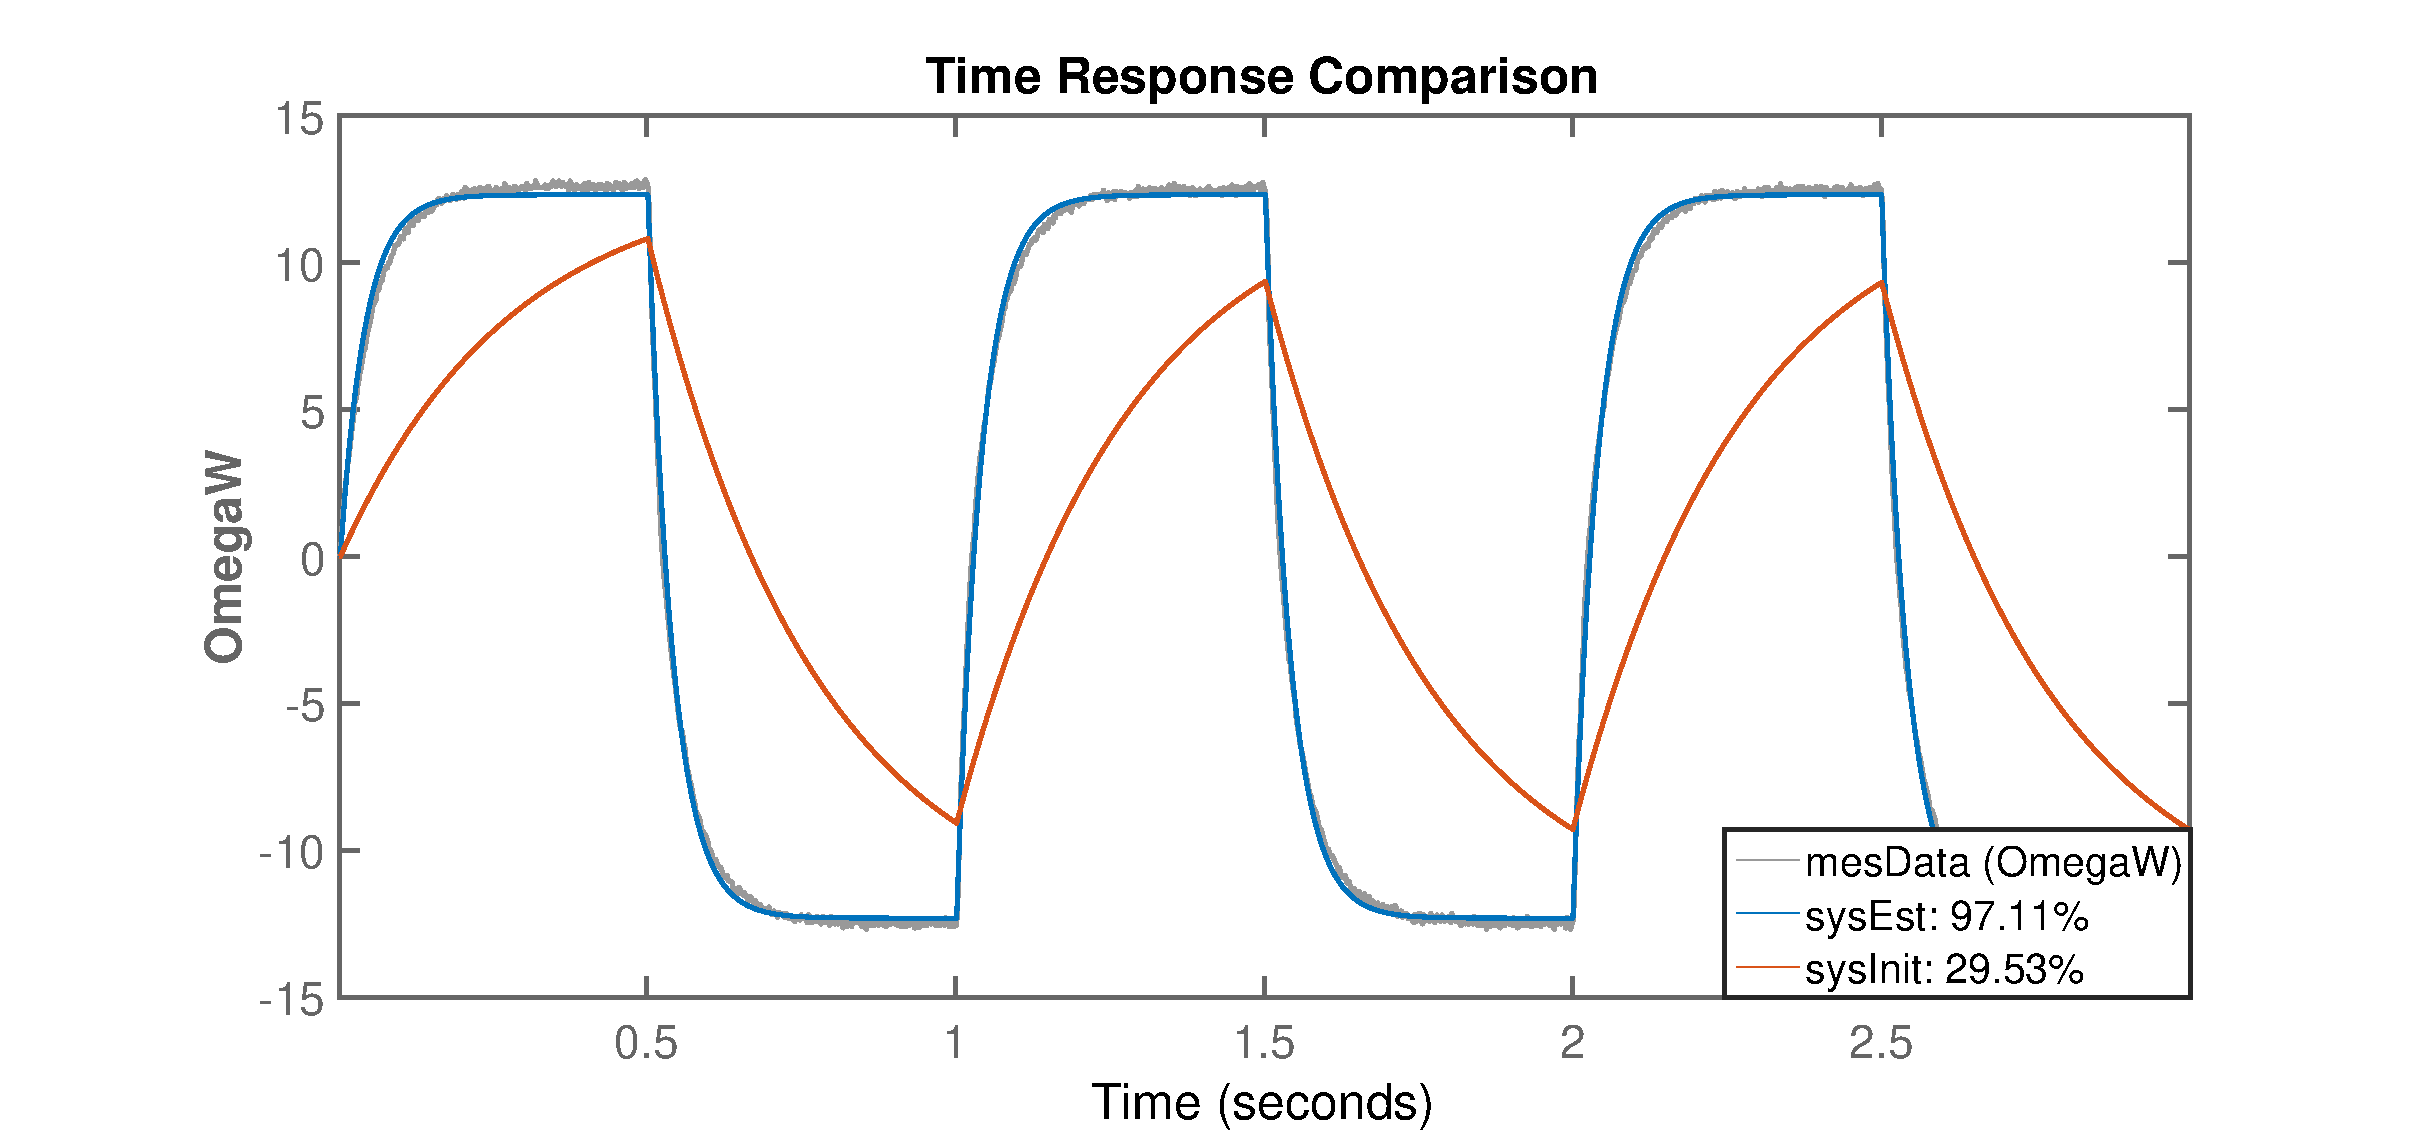
\includegraphics[width = \textwidth]{ParameterEstimation.eps}
    \caption{Bode plot of the transfer function for the segway.}
    \label{fig:paramEst1}
\end{figure} 

With the new gain, the response can be seen in \autoref{fig:paramEst1}, where the model prediction, shown in orange, is shown together with the measured data in grey. The blue axis is Matlab's estimate, based on the model type and measured data.

The model provided by matlab is tested on a different data set, where the motor voltage is changed from 1,96 V to -3,92 V. This can be seen in \autoref{fig:segwayBode_Merge}, where a correlation between the model and the data of $83 \% $ is obtained.

\begin{figure}[H]
    \centering
    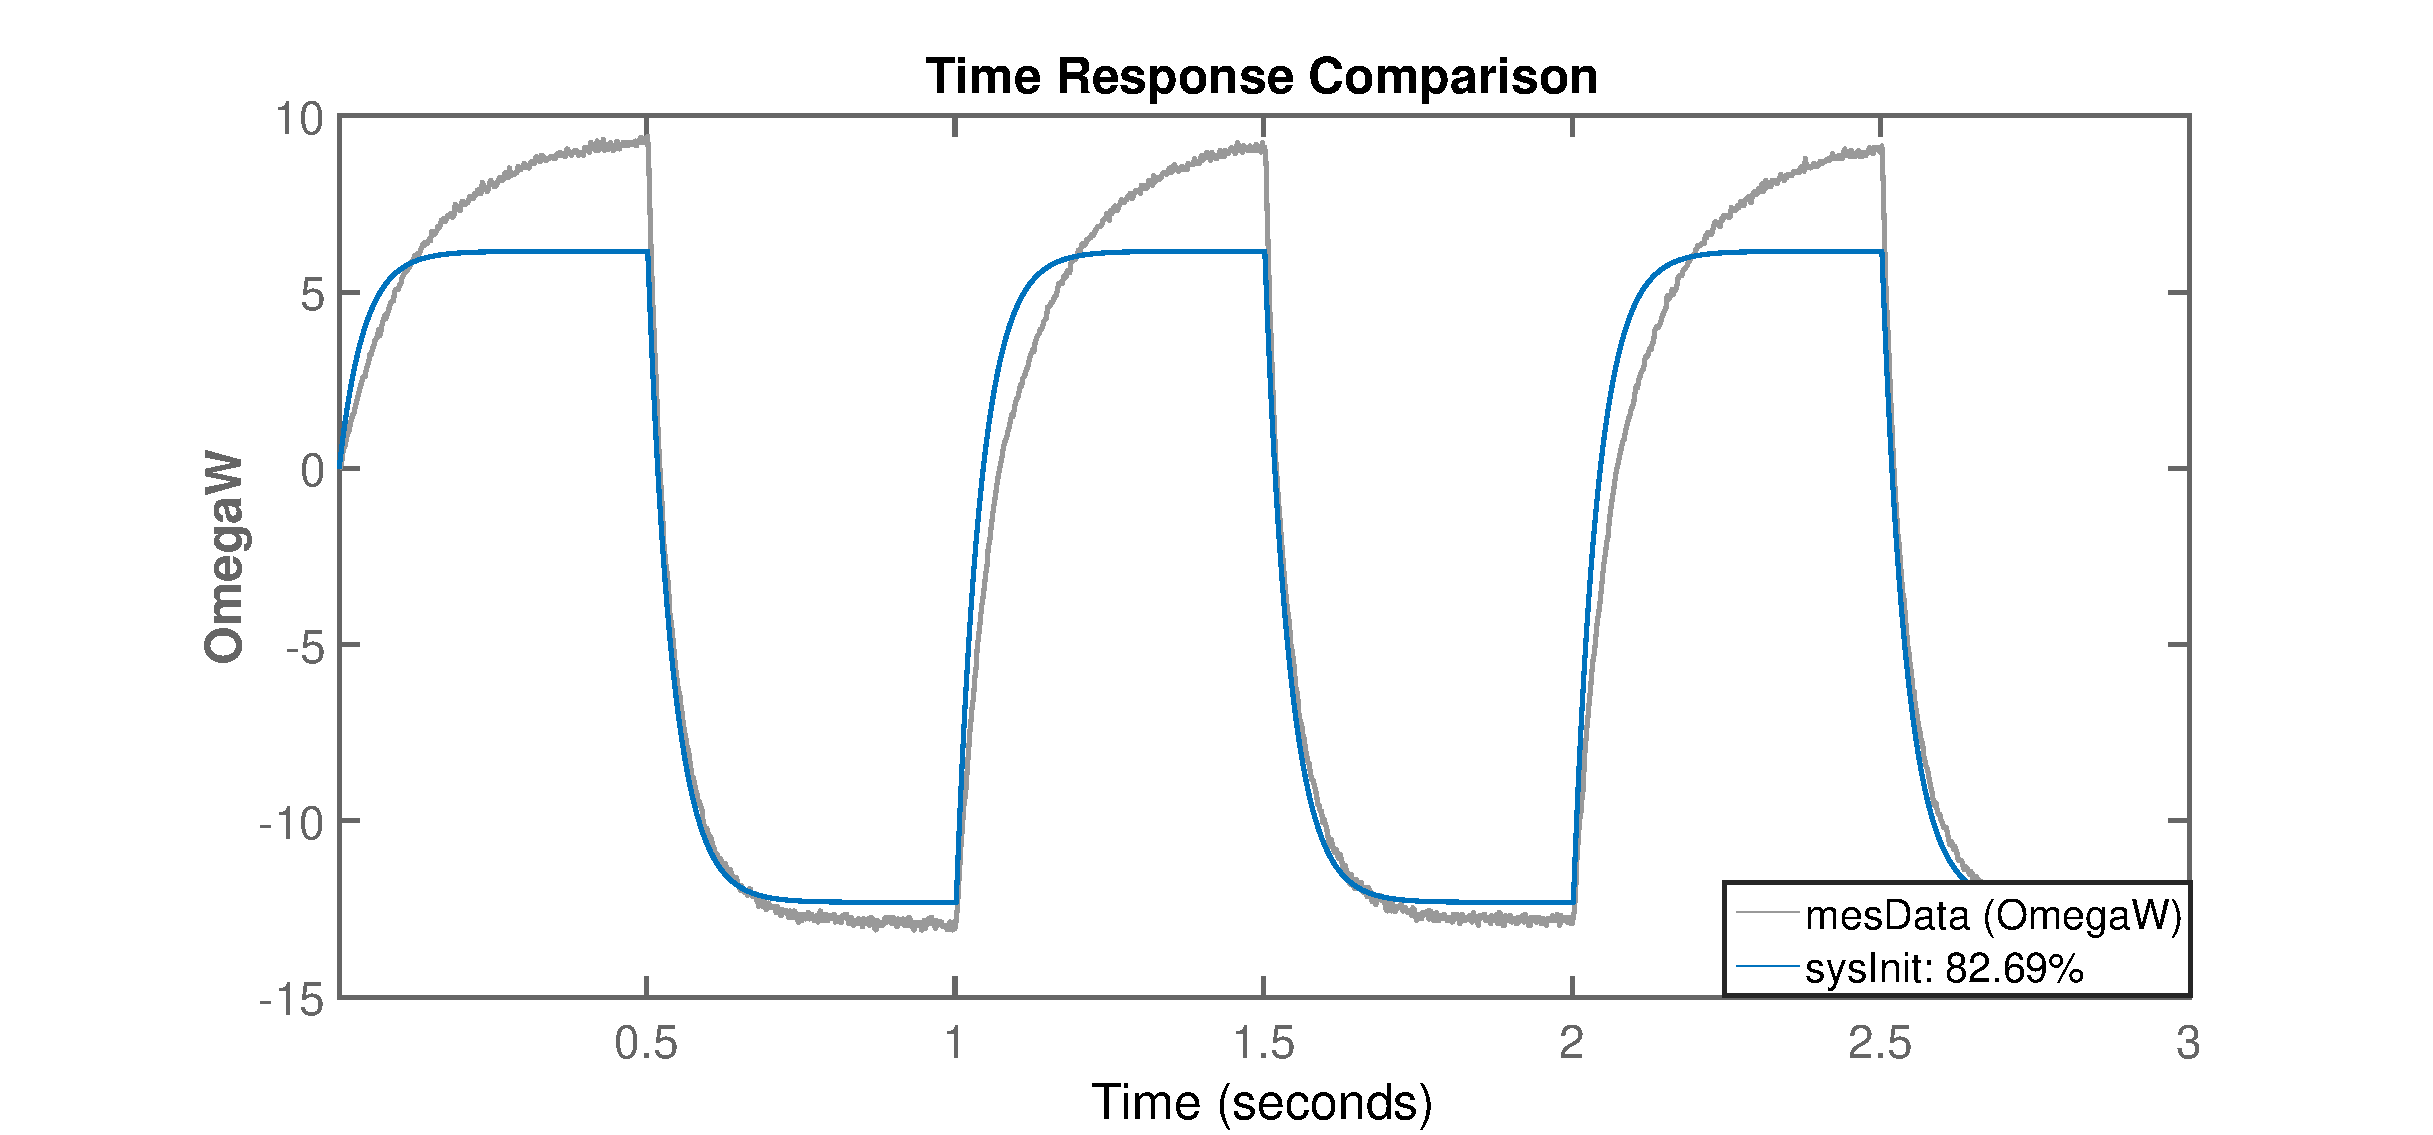
\includegraphics[width = \textwidth]{EstimationTest.eps}
    \caption{Bode plot of the transfer function for the segway.}
    \label{fig:paramEst2}
\end{figure} 

This is assumed to be satisfying, and thus the model for the motors and wheels has been found. Note that in the test, it is the transfer function $\frac{\omega_w{s}}{V_a(s)}$ that has been found, and thus the relationship between $\omega_w$ and $F_F$ as stated in \autoref{OmegaToForce} has to be taken into account. Doing this, results in the following transfer function:

\begin{equation}
\frac{F_F(s)}{V_a(s)} = \frac{0.049s}{0.040s + 1}
\label{eq:motorWheelFinal}
\end{equation}

